\documentclass[tikz,border=10pt]{standalone}
\usepackage{pgfplots}
\usepackage{tikz}
\usepackage{amsmath}

\begin{document}

\centering
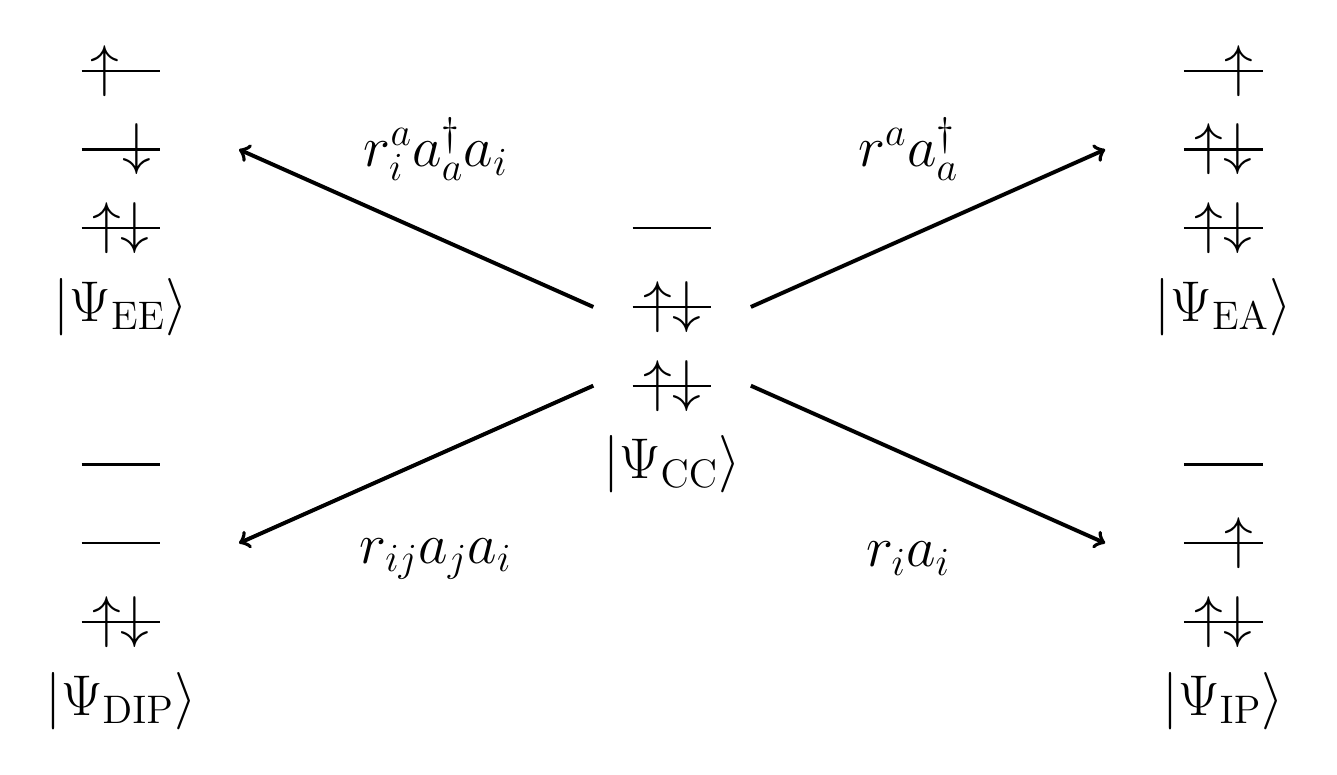
\begin{tikzpicture}
    \huge
    % Define styles
    \tikzset{
        level/.style={thick},
        arrow/.style={->, thick},
        label/.style={font=\small}
    }

    % Draw CC wavefunction levels (left)
    \draw[level] (-4,2) -- (-3,2); 
    \draw[level] (-4,1) -- (-3,1);
    \draw[level] (-4,0) -- (-3,0);
    % Draw electron occupancies for CC
    \node at (-3.5,0) {\(\uparrow\downarrow\)};
    \node at (-3.5,1) {\(\uparrow\downarrow\)};
    % Label CC wavefunction
    \node[label] at (-3.5,-1) {\huge$|\Psi_{\text{CC}}\rangle$};

    % Draw EA wavefunction levels (right)
    \draw[level] (3,4) -- (4,4);
    \draw[level] (3,3) -- (4,3);
    \draw[level] (3,2) -- (4,2);
    % Draw electron occupancies for EA
    \node at (3.7,4) {\(\uparrow\)};
    \node at (3.5,3) {\(\uparrow\downarrow\)};
    \node at (3.5,2) {\(\uparrow\downarrow\)};
    % Label EA wavefunction
    \node[label] at (3.5,1) {\huge$|\Psi_{\text{EA}}\rangle$};
    % Draw transition arrow and label
    \draw [->,line width=0.5mm] (-2.5,1) -- (2,3);
    \node[label] at (-0.5,3) {\huge$r^a a^\dagger_a$};

    % Draw EE wavefunction levels (right)
    \draw[level] (-11,4) -- (-10,4);
    \draw[level] (-11,3) -- (-10,3);
    \draw[level] (-11,2) -- (-10,2);
    % Draw electron occupancies for EE
    \node at (-10.7,4) {\(\uparrow\)};
    \node at (-10.3,3) {\(\downarrow\)};
    \node at (-10.5,2) {\(\uparrow\downarrow\)};
    % Label EE wavefunction
    \node[label] at (-10.5,1) {\huge$|\Psi_{\text{EE}}\rangle$};
    % Draw transition arrow and label
    \draw [->,line width=0.5mm] (-4.5,1) -- (-9,3);
    \node[label] at (-6.5,3) {\huge$r^a_i a^\dagger_a a_i$};

    % Draw DIP wavefunction levels (right)
    \draw[level] (-11,-1) -- (-10,-1);
    \draw[level] (-11,-2) -- (-10,-2);
    \draw[level] (-11,-3) -- (-10,-3);
    % Draw electron occupancies for DIP
    \node at (-10.5,-3) {\(\uparrow\downarrow\)};
    % Label DIP wavefunction
    \node[label] at (-10.5,-4) {\huge$|\Psi_{\text{DIP}}\rangle$};
    % Draw transition arrow and label
    \draw [->,line width=0.5mm] (-4.5,0) -- (-9,-2);
    \node[label] at (-6.5,-2.2) {\huge$r_{ij} a_j a_i$};

    % Draw IP wavefunction levels (right)
    \draw[level] (3,-1) -- (4,-1);
    \draw[level] (3,-2) -- (4,-2);
    \draw[level] (3,-3) -- (4,-3);
    % Draw electron occupancies for IP
    \node at (3.7,-2) {\(\uparrow\)};
    \node at (3.5,-3) {\(\uparrow\downarrow\)};
    % Label IP wavefunction
    \node[label] at (3.5,-4) {\huge$|\Psi_{\text{IP}}\rangle$};
    % Draw transition arrow and label
    \draw [->,line width=0.5mm] (-2.5,0) -- (2,-2);
    \node[label] at (-0.5,-2.2) {\huge$r_i a_i$};

\end{tikzpicture}

\end{document}
